%%%%%%%%%%%%%%%%%%%%%%%%%%%%%%%%%%%%%%%%%%%%%%%%%%%%%%%%%%
%                                                                                      %
%         Bristol Project LaTex Template            %
%                                                                                      %
%%%%%%%%%%%%%%%%%%%%%%%%%%%%%%%%%%%%%%%%%%%%%%%%%%%%%%%%%%
%
%   Author: Alex Charles           Email: aep.charles@gmail.com
%
% -----------------------------------------------------------------------------------
%      PACKAGES & OTHER DOCUMENT CONFIGURATIONS
% -----------------------------------------------------------------------------------
\documentclass[11pt]{article}
\usepackage[utf8]{inputenc}
\usepackage[T1]{fontenc}
\usepackage[british]{babel}
% ----------NEW BIBLATEX BIBLIOGRAPHY-----------------------------------------------
\usepackage[backend=bibtex,style = ieee]{biblatex} % Upgrades Bibliography

\addbibresource{BibFile.bib} %%% For biblatex
%e.g to add page number \footfullcite[chapter, p.~215]{AAIB}
% This allows can use footfullcite commands
% Note urldate field must be in yyyy-mm-dd to work - use online type
% Remeber to use \printbibliography in the footer
% -----------------------------------------------------------------------------------
\usepackage{sectsty}
\usepackage{amssymb,amsmath}
\usepackage{ifxetex,ifluatex}  %<<<<<<<<< Edit FONT HERE
\ifnum 0\ifxetex 1\fi\ifluatex 1\fi=0 % if pdftex
  \usepackage[T1]{fontenc}
  \usepackage[utf8]{inputenc}
\else % if luatex or xelatex
  \ifxetex
    \usepackage{mathspec}
    \setmainfont{Avenir-Light}
  \else
  % Font Package for XeLatex
    \usepackage{fontspec}
    \setmainfont{Avenir-Light}
  \fi
  \defaultfontfeatures{Ligatures=TeX,Scale=MatchLowercase}
\fi
\usepackage[fit]{truncate} %Truncates headers that are too long
\usepackage{fancyhdr}
\usepackage{lastpage}
\usepackage{extramarks}
\usepackage{gensymb}
\usepackage{lipsum}
\usepackage{float}
\usepackage{graphicx}
\graphicspath{{TempImg/}{Img/}}%<<<<<<<<< Location of Template Images and Other Images, Add folders here
\usepackage{subfig}
\usepackage{wrapfig}
\usepackage[font ={small,it}]{caption}
\usepackage{amsfonts,amsthm} % Math packages
% \usepackage{cite}
% \usepackage[maxlevel=3]{csquotes}
%    \MakeAutoQuote{‘}{’}
%    \MakeAutoQuote*{“}{”} %corrects quote marks
\usepackage{enumitem} % resume numbered lists
\usepackage{multicol} %for mulitple colums in lists
\usepackage{geometry}
\usepackage{booktabs} %<<<<<<<<< Table drawing package
\usepackage[table,xcdraw]{xcolor} %<<<<<<<<< Table drawing package
\usepackage{svg}
\usepackage{scrextend} %call footnotes
\usepackage[colorlinks, linkcolor = black, citecolor = black, filecolor = black, urlcolor = blue]{hyperref} % Creates Hyperlinks for references - add [colorlinks] for coloured hyperlinks
\usepackage{changepage} %Allows Adjust width to be used for the document (indenting paragraphs)
\usepackage{pdfpages} %Allows Pdfpages to be added to the document use \includepdf[pages={1}]{myfile.pdf}
\usepackage{pdflscape} %Change Pages from Portrait to Landscape

%\usepackage[compact]{titlesec}
\usepackage{titlesec}
\titlespacing\section{0pt}{8pt plus 4pt minus 2pt}{0pt plus 2pt minus 2pt}
\titlespacing\subsection{0pt}{0pt plus 3pt minus 2pt}{-3pt plus 2pt minus 2pt}
\titlespacing\subsubsection{0pt}{0pt plus 2pt minus 2pt}{-6pt plus 2pt minus 2pt}
\titlespacing\subsubsubsection{0pt}{-6pt plus 2pt minus 2pt}{-6pt plus 2pt minus 2pt}
\setlength{\multicolsep}{-1pt plus 2.0pt minus 1.5pt}% 50% of original values

% \titlespacing*{\section}{0pt}{1.1\baselineskip}{\baselineskip}

\renewcommand*{\thefootnote}{\alph{footnote}} %%% Changes footnotes to letters
\usepackage[bottom]{footmisc} %%% Pushes footnote to bottom and to the margin

\DeclareCiteCommand{\footcite}[\mkbibfootnote]
{\usebibmacro{cite:init}%
\usebibmacro{prenote}}
{\usebibmacro{citeindex}%
\printtext[brackets]{\usebibmacro{cite:comp}}}
{\multicitedelim}
{\usebibmacro{cite:dump}%
\usebibmacro{postnote}}

\newenvironment{indentpara}{\begin{adjustwidth}{2cm}{}}{\end{adjustwidth}} %Declare adjust width wiht indentpara
\renewcommand{\labelitemii}{$\circ$}
\renewcommand{\labelitemiii}{$\diamond$}
\renewcommand{\labelitemiii}{$\cdot$}

% -----------------------------------------------------------------------------------
%                 Code
% -----------------------------------------------------------------------------------
\usepackage{listings}
\lstset{inputpath=Code/}
\usepackage{color}
\definecolor{mygreen}{RGB}{28,172,0} % color values Red, Green, Blue
\definecolor{mylilas}{RGB}{170,55,241}

\lstset{language=Matlab,%
    %basicstyle=\color{red},
    breaklines=true,%
    basicstyle=\small,
    morekeywords={matlab2tikz},
    keywordstyle=\color{blue},%
    morekeywords=[2]{1}, keywordstyle=[2]{\color{black}},
    identifierstyle=\color{black},%
    stringstyle=\color{mylilas},
    commentstyle=\color{mygreen},%
    showstringspaces=false,%without this there will be a symbol in the places where there is a space
    numbers=left,%
    numberstyle={\tiny \color{black}},% size of the numbers
    numbersep=9pt, % this defines how far the numbers are from the text
    emph=[1]{for,end,break},emphstyle=[1]\color{red}, %some words to emphasise
    %emph=[2]{word1,word2}, emphstyle=[2]{style},
}

%% To Add Code Use :
% \lstinputlisting{myfun.m}
%% To input a file or :
% \begin{figure}[h]
% \begin{lstlisting}[language=Matlab]
% \end{lstlisting}
% \catpion{code}
% \end{figure}


% -----------------------------------------------------------------------------------
%                 Quotes
% -----------------------------------------------------------------------------------

\usepackage{epigraph}
% \epigraphsize{\small}% Default
\setlength\epigraphwidth{12cm}
\setlength\epigraphrule{0pt}

\usepackage{etoolbox}
\apptocmd{\sloppy}{\hbadness 10000\relax}{}{}%%%% > Removes Url bibliography warnings
\makeatletter
\patchcmd{\epigraph}{\@epitext{#1}}{\itshape\@epitext{#1}}{}{}
\makeatother

%%%% > For Quotes Use \epigraph{"Quote"}{ - \textup{Author}, Book}

% -----------------------------------------------------------------------------------
%                   NAMES & CLASS DEFINITION %<<<<<<<<< INSERT DETAILS HERE
% -----------------------------------------------------------------------------------
\newcommand{\AssignmentTitle}{Part 1: Identification of Transfer Functions}
\newcommand{\ModuleTitle}{Sensors, Signals and Control}
\newcommand{\University}{University of Bristol}
\newcommand{\Faculty}{Faculty of Engineering}
\newcommand{\UniCrest}{crestbris.png}
\newcommand{\UniLogo}{logobris.png}%<<<<<<<<< Make Sure Files are in the Template
%\newcommand{\GroupName}{Group 2}
\newcommand{\StudentNameA}{Alex Charles}
\newcommand{\StudentNumberA}{ac13625}
\newcommand{\StudentNameB}{Akash Ramineni}
\newcommand{\StudentNumberB}{ar14120}
\newcommand{\SupervisorNameA}{Andres Marcos}
\newcommand{\SupervisorEmailA}{Andres.Marcos@bristol.ac.uk}
\newcommand{\SupervisorNameB}{Name}
\newcommand{\SupervisorEmailB}{email@gmail.com}

% -----------------------------------------------------------------------------------
%        PACKAGES FOR MARKDOWN CONVERSION - FOR USE If Using Markdown to Latex
% -----------------------------------------------------------------------------------
\usepackage{fixltx2e} % provides \textsubscript
% use upquote if available, for straight quotes in verbatim environments
\IfFileExists{upquote.sty}{\usepackage{upquote}}{}
% use microtype if available
\IfFileExists{microtype.sty}{%
\usepackage{microtype}
\UseMicrotypeSet[protrusion]{basicmath} % disable protrusion for tt fonts
}{}
\hypersetup{unicode=true,
            pdftitle={\AssignmentTitle},
            pdfauthor={\StudentNameA},
            pdfborder={0 0 0},
            breaklinks=true}
\urlstyle{same}  % don't use monospace font for urls
\usepackage{fancyvrb}
\VerbatimFootnotes % allows verbatim text in footnotes
\usepackage{longtable,booktabs}
\IfFileExists{parskip.sty}{%
\usepackage{parskip}
}{% else
\setlength{\parindent}{0pt}s
\setlength{\parskip}{6pt plus 2pt minus 1pt}
}
\setlength{\emergencystretch}{3em}  % prevent overfull lines
\providecommand{\tightlist}{%
  \setlength{\itemsep}{0pt}\setlength{\parskip}{0pt}}
% \setcounter{secnumdepth}{0}
% Redefines (sub)paragraphs to behave more like sections
\ifx\paragraph\undefined\else
\let\oldparagraph\paragraph
\renewcommand{\paragraph}[1]{\oldparagraph{#1}\mbox{}}
\fi
\ifx\subparagraph\undefined\else
\let\oldsubparagraph\subparagraph
\renewcommand{\subparagraph}[1]{\oldsubparagraph{#1}\mbox{}}
\fi

% -----------------------------------------------------------------------------------
%                   WORD COUTNER - for XeLaTex
% -----------------------------------------------------------------------------------
\usepackage{xesearch}
\newcounter{words}
\newenvironment{counted}{%
  \setcounter{words}{0}
  \SearchList!{wordcount}{\stepcounter{words}}
    {a?,b?,c?,d?,e?,f?,g?,h?,i?,j?,k?,l?,m?,
    n?,o?,p?,q?,r?,s?,t?,u?,v?,w?,x?,y?,z?}
  \UndoBoundary{'}
  \SearchOrder{p;}}{%
  \StopSearching}

% -----------------------------------------------------------------------------------
%                   MARGINS, HEADERS & FOOTERS
% -----------------------------------------------------------------------------------
 \geometry{
 left=20mm,
 right=20mm,
 top=20mm,
 bottom=20mm,
 }
\linespread{1.05}

\pagestyle{fancy}
\lhead{\includegraphics[width = 0.2\textwidth]{\UniLogo}}
% \chead{\AssignmentTitle}
% \rhead{}
\lfoot{\StudentNameA, \StudentNameB}
\cfoot{}
\rfoot{Page \thepage} %%%% note the footer is swapped when page numbering style changes
\renewcommand\headrulewidth{0.4pt}
\renewcommand\footrulewidth{0.4pt}

\setlength\parindent{0pt}

\newcommand{\horrule}[1]{\rule{\linewidth}{#1}}

% -----------------------------------------------------------------------------------
%               DOCUMENT STRUCTURE COMMANDS
% -----------------------------------------------------------------------------------
% To sort out the formatting of header and footer when a page...
% ... split occurs "within" a problem environment.
\newcommand{\enterProblemHeader}[1]{
\nobreak\extramarks{#1 (Cont.)}\nobreak
\nobreak\extramarks{#1}{}\nobreak
}
% To sort out the formatting of header and footer when a page...
% ... split occur "between" problem environments.
\newcommand{\exitProblemHeader}[1]{
\nobreak\extramarks{#1 (Cont.)}\nobreak
\nobreak\extramarks{#1}{}\nobreak
}

% -----------------------------------------------------------------------------------
\begin{document}

  \setlength{\abovedisplayskip}{-18pt}
  \setlength{\belowdisplayskip}{0pt}
  \setlength{\abovedisplayshortskip}{-18pt}
  \setlength{\belowdisplayshortskip}{0pt}

  \setlist[enumerate]{itemsep=-2mm}
  \setlist[itemize]{itemsep=-2mm}


%----------------------------------------------------------------------------------------
                                  %	TITLE PAGE FORMAT
%----------------------------------------------------------------------------------------
\pagenumbering{roman}
\begin{titlepage}

	\center % Center everything on the page
%----------------------------------------------------------------------------------------
%	HEADING SECTION
%----------------------------------------------------------------------------------------
		\usefont{OT1}{bch}{b}{n}
		\normalfont \normalsize \textsc{\University} \\ [10pt]
		\normalfont \normalsize \textsc{\Faculty} \\ [25pt]
%----------------------------------------------------------------------------------------
%	LOGO SECTION - Adds Univeristy Crest to the Report
%----------------------------------------------------------------------------------------
		\includegraphics[width = 0.2\textwidth]{\UniCrest}\\[0.5cm]
%----------------------------------------------------------------------------------------
%	HEADING SECTION
%----------------------------------------------------------------------------------------
		\normalfont \normalsize \textsc{\ModuleTitle} \\ [25pt]
%----------------------------------------------------------------------------------------
%	TITLE SECTION
%----------------------------------------------------------------------------------------
		\horrule{0.5pt} \\[0.4cm]
		\huge \textbf{\AssignmentTitle} \\
		\horrule{2pt} \\[0.5cm]
%----------------------------------------------------------------------------------------
%	HEADING SECTION
%----------------------------------------------------------------------------------------
%		\normalfont \normalsize \textsc{\GroupName} \\ [25pt]
%----------------------------------------------------------------------------------------
%	AUTHOR SECTION
%----------------------------------------------------------------------------------------
\begin{minipage}{0.4\textwidth}
\begin{flushleft} \large
\emph{Supervisors:}\\
% Change Name
\textbf{\SupervisorNameA}\\
% \textbf{\SupervisorNameB}
\end{flushleft}
\end{minipage}
~
\begin{minipage}{0.4\textwidth}
\begin{flushright} \large
\emph{Email:} \\
\SupervisorEmailA\\
% \SupervisorEmailB

\end{flushright}
\end{minipage}\\[1cm]

\begin{minipage}{0.4\textwidth}
\begin{flushleft} \large
\emph{Authors:}\\
	\textbf{\StudentNameA}\\
  \textbf{\StudentNameB}
\end{flushleft}
\end{minipage}
~
\begin{minipage}{0.4\textwidth}
\begin{flushright} \large
\emph{Candidate Number:} \\
(\StudentNumberA)\\
(\StudentNumberB)
\end{flushright}
\end{minipage}\\[2cm]

%----------------------------------------------------------------------------------------
%	DATE SECTION
%----------------------------------------------------------------------------------------
\textit{{\large \today}}\\[1cm] % Date, change the \today to a set date if you want to be precise
%----------------------------------------------------------------------------------------
\vfill % Fill the rest of the page with whitespace
\end{titlepage}

% \setcounter{page}{3}

\newpage


% -----------------------------------------------------------------------------------
%                             	 ABSTRACT
% -----------------------------------------------------------------------------------

% \addcontentsline{toc}{section}{Abstract}
% \begin{abstract}
%
% \end{abstract}
% -----------------------------------------------------------------------------------
%                              TABLE OF CONTENTS
% -----------------------------------------------------------------------------------

% \tableofcontents


% \newpage

% \addcontentsline{toc}{section}{List of Tables}
% \listoftables
% \addcontentsline{toc}{section}{List of Figures}
% \listoffigures
% \addcontentsline{toc}{section}{List of Acronyms}
% \section*{List of Acronyms}\label{acronyms}
% \textbf{BRB}: Be Right Back \\


% \newpage

% \addcontentsline{toc}{section}{Acknowledgements}
% \section*{Acknowledgements}\label{acknowledgements}

% \addcontentsline{toc}{section}{Declaration}
% \section*{Declaration}\label{declartion}
% I hereby declare that this report entitled “\AssignmentTitle” submitted to Bristol University, is a record of an original work completed by myself.\\

% \newpage

%% -----------------------------------------------------------------------------------
%%                          	  INTRODUCTION
%% -----------------------------------------------------------------------------------
\clearpage
\rfoot{Page \thepage\ of \pageref{LastPage}}
\pagenumbering{arabic}
\begin{counted} %<<<<<<<<<<<<<<STARTS WORD COUNTER
\section{Introduction and Open Loop
Discussion}\label{introduction-and-open-loop-discussion}

\begin{wrapfigure}{r}{0.62\textwidth}
  \begin{center}
  \vspace{-20pt}
  \includegraphics[trim = 150 60 180 20, clip, width=0.615\textwidth]{intrograph.pdf}
  \end{center}
  \caption{Graph Showing the Open Loop Nature of the Experimental Quanser Response}
  \label{intrograph}
  \vspace{-15pt}
\end{wrapfigure}

This report compares the experimental and theoretical transfer functions
of 3 degree of freedom Quanser-Control rig. Control design is important
to understand the behaviour of a dynamic system, and then improve the
performance. Sensors and actuators are used in the Quanser to measure
and vary performance characteristics of the Quanser. In this case, an
elevation change was introduced to the Quanser in order to observe an
oscillating damped behaviour. Measuring this response a theoretical
transfer function was then estimated.

An Open-Loop system is a where behavioural characteristics can be
controlled manually. These changes are not feedback into the system,
therefore the output has no effect on the input of the system
\cite{openloop} meaning self-correction is not possible. In the case of
the Quanser-Control Rig, elevation angle was independent of the output
and manually controlled, whereas pitch and travel data was manually
feedback to the system. Figure \ref{intrograph} shows the open loop
behaviour of the elevation axis, as the elevation angle was varied
between 10 and 40 degrees.

\section{Method and Results}\label{method-and-results}

\subsection{Finding Experimentation Results from
Quansers}\label{finding-experimentation-results-from-quansers}

\begin{enumerate}
  \item
    \parbox[t]{\dimexpr\textwidth-\leftmargin}{%
      \vspace{-3mm}
      \begin{wrapfigure}{r}{0.6\textwidth}
      \vspace{-10pt}
        \centering
        \captionof{table}{Table Showing Key Parameter Calculations \cite{vibnote},\cite{vibnote2}}
\includegraphics[trim = 0 0 0 0, clip, width=\linewidth]{eqtable.pdf}
\label{eqtable}
\vspace{-25pt}
      \end{wrapfigure}
      Replace the elevator input with a step block, using the parameters: Start Time: 40s, Start Value: -2, End Value: -1 to 2. This was used to automate the step input at a specific time for each elevator input test. A step input time of 40s was chosen to allow the initial response to settle to an acceptable level (see Figure \ref{intrograph}).
      \vspace{3mm}
      \item Use range of elevator input values, varying from an initial value of -2 to 2 in steps of 1. Repeat each test case, saving workspace variables.
      \vspace{3mm}
      \item Check data for anomalies, Averaged repeats for valid results across the different step inputs.
    }
  \end{enumerate}

\subsection{Analyse Transfer Function}\label{analyse-transfer-function}

\begin{enumerate}

\item
  Isolate elevation values for corresponding inputs from 40s to 80s;
  this captures this captures the response after step input.
\item
  In order to estimate a transfer function - the following parameters
  were calculated: Natural frequency, Undamped natural frequency and
  damping ratio, refer to Table \ref{eqtable}.
\end{enumerate}

\subsubsection{Second Order}\label{second-order}

To calculate the Second Order Transfer-Function, a forced response
behaviour was noted. Using Table \ref{eqtable} equations \cite{vibnote}
\cite{vibnote2}, in addition to the x and y values taken from the peaks
highlighted in figure \ref{intrograph} the logarithmic decrement and the
period of damp oscillation was approximated. Using these equations
values for the damping ratio \(\zeta\) and natural frequency
\(\omega_n\) were obtained and substituted into the formal equation
shown in equation \ref{2otf}.

\begin{align}
\frac{ y(s) }{ u(s) } &=\frac{ k\cdot \omega_{ n }^{ 2 } }{ s^{ 2 }+2\zeta \omega_{ n }s+\omega_{ n }^{ 2 } } \label{2otf}
\end{align}

In order to obtain a single transfer function which represents the
system as a whole for varying elevators angle steps, estimated transfer
functions were found for each test case. These parameters were then
averaged obtaining a single fit transfer function where gain was changed
to model different elevator angle step inputs. This captured some of the
behaviour of the system as step level varied.

\begin{wrapfigure}{r}{0.5\textwidth}
  \begin{center}
  \vspace{-20pt}
\includegraphics[trim = 10 10 10 10, clip, width=0.49\textwidth]{kgraph.pdf}  
\end{center}
\caption{Graph Finding the Gain For Each Step Input}
\label{kgraph}
  \vspace{-15pt}
\end{wrapfigure}

To calculated the a representative gain scaling factor \(k\) for each of
the step inputs, max elevation for each step input was taken (from the
first peak shown in Figure \ref{intrograph}). These values were plotted
on a graph to find their correlation, shown in figure \ref{kgraph}. The
gain \(k\) value was heuristically adjusting to match the estimated
amplitude with the experimental results from -2 to 2, where it was found
that \(k = 0.26\). This value was used to translate the correlation
equation between points into scaling factors.

After applying this method, amplitudes for all the steps fitted more
closely. Finally damping ratio and undamped natural frequency were
tweaked to give the final fit, again by trial and error.

\subsubsection{First Order}\label{first-order}

Standard First Order Response Transfer Function:

\begin{align}
 \frac { y(s) }{ u(s) } &=\frac { k }{ \tau s+1 }
\label{fos}
\end{align}

Due to the Quanser-Control Rig being a Second Order System Equation
\ref{fos} was not applicable for finding the First Order Transfer
Function. Instead this was estimated by considering the Second Order
Transfer Function case where: \(\zeta =1\) and \(s^2=0\).

\begin{align}
\frac { k\cdot \omega_{ n }^{ 2 } }{ 2\zeta \omega_{ n }s+\omega_{ n }^{ 2 } } &\rightarrow \frac { k\cdot \omega_{ n }^{ 2 } }{ 2\omega_{ n }s+\omega_{ n }^{ 2 } }
\end{align}

\section{Results}\label{results}

\begin{align}
&\text{2nd Order Transfer Function}: && k \cdot \frac { 1.109 }{ s^{ 2 }+0.1313s+1.109 }
\end{align}

\begin{align*}
\\
&\text{Where:} &&\zeta = 0.0623 &&& \omega_n = 1.0532
\\
\end{align*}

\begin{align}
&\text{1st Order Transfer Function}: && k \cdot \frac { 1.109 }{ 2.106s+1.109 }
\end{align}

\begin{align*}
\\
&\text{Where:} &&\zeta = 1 &&& \omega_n = 1.0532
\\
\end{align*}

\begin{figure}[H]
\centering
\begin{minipage}{.49\textwidth}
\centering
\includegraphics[trim = 35 16 35 0, clip, width=0.995\textwidth]{2ndTFcomp.eps}
\caption{2nd Order Simualted Transfer Function Comparision}
\label{2ndTFcomp}
\end{minipage}
\hfill
\begin{minipage}{.49\textwidth}
  \centering
  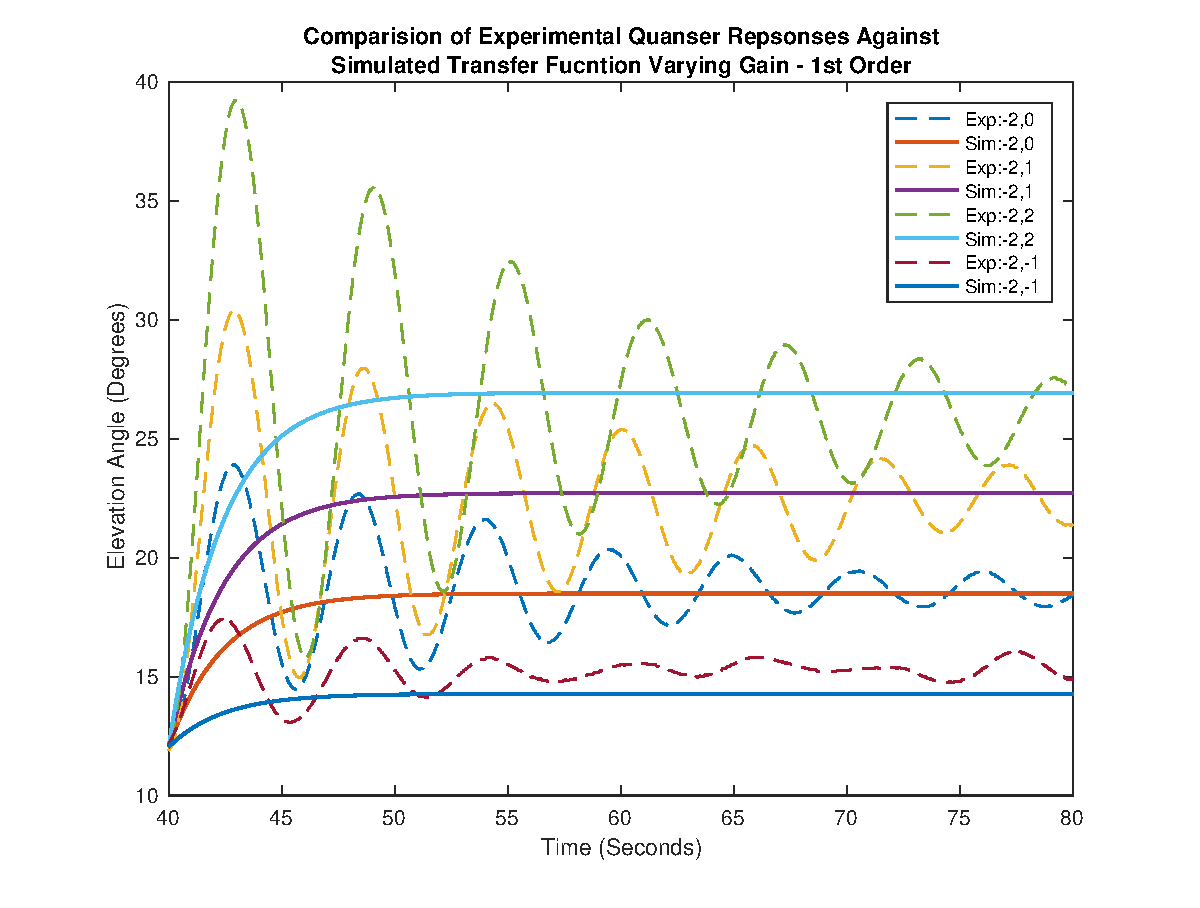
\includegraphics[trim = 35 16 35 0, clip, width=0.995\textwidth]{1stTFcomp.eps}
  \caption{1st Order Simualted Transfer Function Comparision}
  \label{1stTFcomp}
\end{minipage}
\vspace{-11pt}
\end{figure}

\begin{figure}[H]
\centering
\begin{minipage}{.49\textwidth}
Second Order Step Information:
\begin{align*}
t_r &= 1.0385 &&t_s = 57.3382
\end{align*}
\end{minipage}
\hfill
\begin{minipage}{.49\textwidth}
First Order Step Information:
\begin{align*}
t_r &= 4.1719 &&t_s = 7.4287
\end{align*}
\end{minipage}
\vspace{-11pt}
\end{figure}

\section{Observations and Analysis:}\label{observations-and-analysis}

\subsection{Experimental Elevator
Input:}\label{experimental-elevator-input}

\begin{itemize}
\tightlist
\item
  There is an observable phase and amplitude deviation, particularly
  after the third peak. The phase shift becomes increasingly out of
  phase as the initial step input is reduced.
\item
  Peak amplitude prediction becomes worse for lower amplitude cases,
  however there is a very good match for 0,1 and 2 test cases first
  three peaks, the k value equation provided a good match. Note this
  equation was set heuristically to a step input of 2.
\item
  The oscillations around the expected steady level were slightly larger
  above the steady state level rather than below. This could be an
  artefact of the Quanser accumulating elevation drift.
\item
  Steady state values match well for an elevator input of 0 and 1,
  however are noticeably different for -1 and 2.
\end{itemize}

\subsection{\texorpdfstring{Root-Locus plot (See Figure
\ref{poleszmap})}{Root-Locus plot (See Figure )}}\label{root-locus-plot-see-figure}

\begin{itemize}
\tightlist
\item
  The grid lines represent lines of constant damping and lines of
  natural frequency
\item
  The Second Order Transfer Function Root-Locus has a pair of points
  with an imaginary axis component (complex root) - This shows the
  stable underdamped nature of the system as \(0<\zeta<1\)
\item
  The First Order Transfer Function Root-Locus diagram point exists
  purely in the real axis component, meaning the function is critically
  damped as expected and stable.
\item
  Increase in gain for the Second Order shows the roots becoming more
  positive and negative in the imaginary axis respectively
\item
  Increase in gain for the First Order shows the root becoming more
  negative along the real axis
\end{itemize}

\section{Discussion}\label{discussion}

\begin{wrapfigure}{r}{0.56\textwidth}
  \begin{center}
  \vspace{-40pt}
  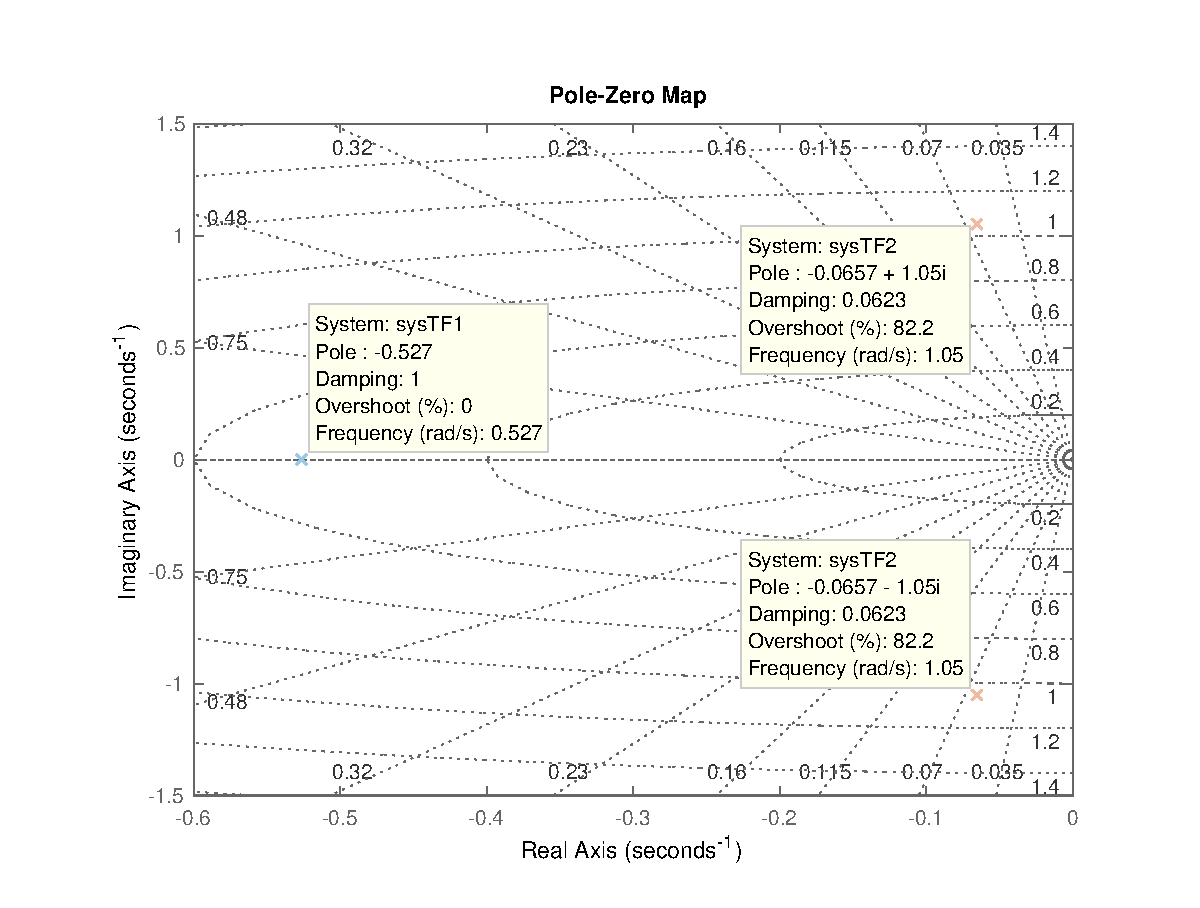
\includegraphics[trim = 35 14 35 0, clip, width=0.55\textwidth]{poleszmap.eps}
  \end{center}
  \caption{Map of the Poles, sysTF1 = First Order, sysTF2 = Second Order}
 \label{poleszmap}
  \vspace{-20pt}
\end{wrapfigure}

Observing Figure \ref{2ndTFcomp} and \ref{1stTFcomp} many deviation's
from MATLAB's theoretical transfer function step response were observed.
During the Quanser operation, a significant observable error was the
drift in the Quanser, more noticeable during longer runs; potentially
due to accumulating error increasing with time. Whilst the Quansers have
error correcting features (through the closed-loop nature of the other
parameters), this is only sensitive to a finite degree so could be
considered imperfect. An initial elevator input was set to -2 (to get
the fans running), and then after 40 seconds an elevator step was input
into the system. As a result the step input may have been applied during
mid oscillation past the steady state elevation position; this likely
either amplified or decreased the actual step input depending on which
stage of oscillation the Quanser was at. A 40 seconds run reduced the
steady-state level to 10-20\% of the steady state value. Errors may
accumulate for a greater run time as the system fails to accurately
correct for inconsistencies.

Another source of deviation is inaccuracy in step input time. In theory
the step input is modelled as an immediate action. A step block was
introduced in the Simulink model to automate the `elevator input' at 40
seconds, however closer observation of the corresponding pitch and
travel data plots revealed a slight delay. Accumulated lag in the system
and controller and a delayed response time both contributed to latency.
Latency causes a phase and amplitude shift in experimental results, as
well as introducing error in parameters such as the logarithmic
decrement \(\Lambda_i\) and damped frequency \(\omega_d\) calculations.

From a mechanical perspective, friction in the Quanser hinge support and
tension from the power cables resulted in a reduction in expected
elevation. This adds to the natural damping of the system, one
explaining for the compacted peaks in experimental data (see Figure
\ref{2ndTFcomp}), and could explain some variation in repeats which was
larger than would be expected for a fixed experiment.

As with any control system, noise can be introduced by external and
internal factors. In the Quanser system, gyro noise and wind resistance
are contributing factors. Sensors in any system measure quantities which
need to be controlled - in this case the elevator sensor sampling was
storing values at discrete points. Whilst the sampling time was quite
small, capturing the general nature of the oscillating damped curves,
some critical points may have been missed. An example can be observed at
the point of highest amplitude, the inflexion behaviour begins after a
region of constant amplitude. Computationally we see a quicker inflexion
transition in this region.

\newpage
% -----------------------------------------------------------------------------------
%                                  APENDIX
% -----------------------------------------------------------------------------------

\end{counted} %<<<<<<<<<<<<<<ENDS WORD COUNTER

\newpage
% \section{Appendices}
Above were \thewords\ words. %<<<<<<<<<<<<<<DISPLAYS WORD COUNTER
% -----------------------------------------------------------------------------------
%                               BIBLIOGRAPHY - Insert Name of BIB File Here
% -----------------------------------------------------------------------------------
% \newpage

% ---------------BIBTEX OLD-----------------------------------------------------
% \bibliographystyle{unsrt} %%%% Plain or alpha can change orders here
% \bibliography{BibFile}
% \nocite{*} %%%if you want to see all references even those note cited in the text
% -----------------------------------------------------------------------------------

\printbibliography

\end{document}
